%-*-EMaxima-*-
\documentclass[12pt,usenames,pdftex]{beamer}

\usetheme{DetlevCM}
\usecolortheme{whale}
\useoutertheme{infolines}

\usepackage[T1]{fontenc}
\usepackage[utf8]{inputenc}
\usepackage{graphics}
\usepackage{lmodern}
\usepackage[lines,breqn]{emaxima}
\usepackage{url}
\usepackage{amsmath}
\usepackage{bm}
\usepackage{listings}
% \usepackage[hidelinks]{hyperref}

\newcommand{\pdderiv}[2][]{\ensuremath{\dfrac{\partial #1}{\partial
      #2}}}

\title[Maxima]{A Tutorial Introduction to Maxima}

\author{Nidish Narayanaa B}

\institute[IIST]
{
  Department of Aerospace Engineering\\
  Indian Institute of Space SCience \& Technology, Trivandrum
}

\date[IISTFOSS, 17]{FOSS Group, IIST, 2017}

% \logo{
\includegraphics[width=\linewidth]{Figs/V0}}
\subject{MaximaTut_IISTFOSS}

\AtBeginSection[]{
  \begin{frame}<beamer>{Outline}
    \tableofcontents[currentsection]{}
  \end{frame}
}

\begin{document}
\maketitle{}
\section{Introduction}

\begin{frame}
  \frametitle{What is Maxima?}
  \begin{quotation}
    (From the website)
    Maxima is a system for the \textbf{manipulation of symbolic and
      numerical expressions}, including differentiation,
      integration, Taylor series, Laplace transforms, ordinary
      differential equations, systems of linear equations,
      polynomials, sets, lists, vectors, matrices and tensors.
  \end{quotation}
\end{frame}

\begin{frame}
  \frametitle{What is Maxima?}
  \begin{itemize}
  \item Powerful Computer Algebra System (CAS) combining symbolic,
    numerical, and graphical capabilities
  \item Cousin of the commercial Macsyma CAS (currently available
    without support)    
  \item Completely Free and Open Source Software, written in LISP
  \item Fully customizable and extensible
  \end{itemize}
\end{frame}

\begin{frame}[<1->]{Interface}
  \frametitle{Interface}
  \begin{columns}
    \begin{column}{0.35\linewidth}
      \begin{description}
      \item<1->[maxima] Native CLI
      \item<2->[xmaxima] History :)
      \item<3->[wxmaxima] Wxwidgets
      \item<4->[imaxima] Emacs!
      \end{description}
    \end{column}
    \begin{column}{0.65\linewidth}
      \begin{center}
        \only<1>{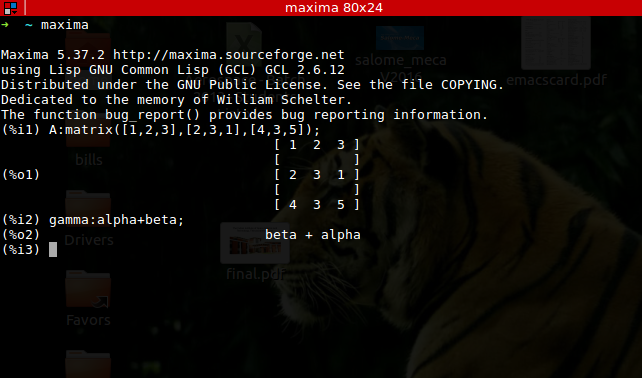
\includegraphics[width=\linewidth]
          {Figs/cli}} 
        \only<2>{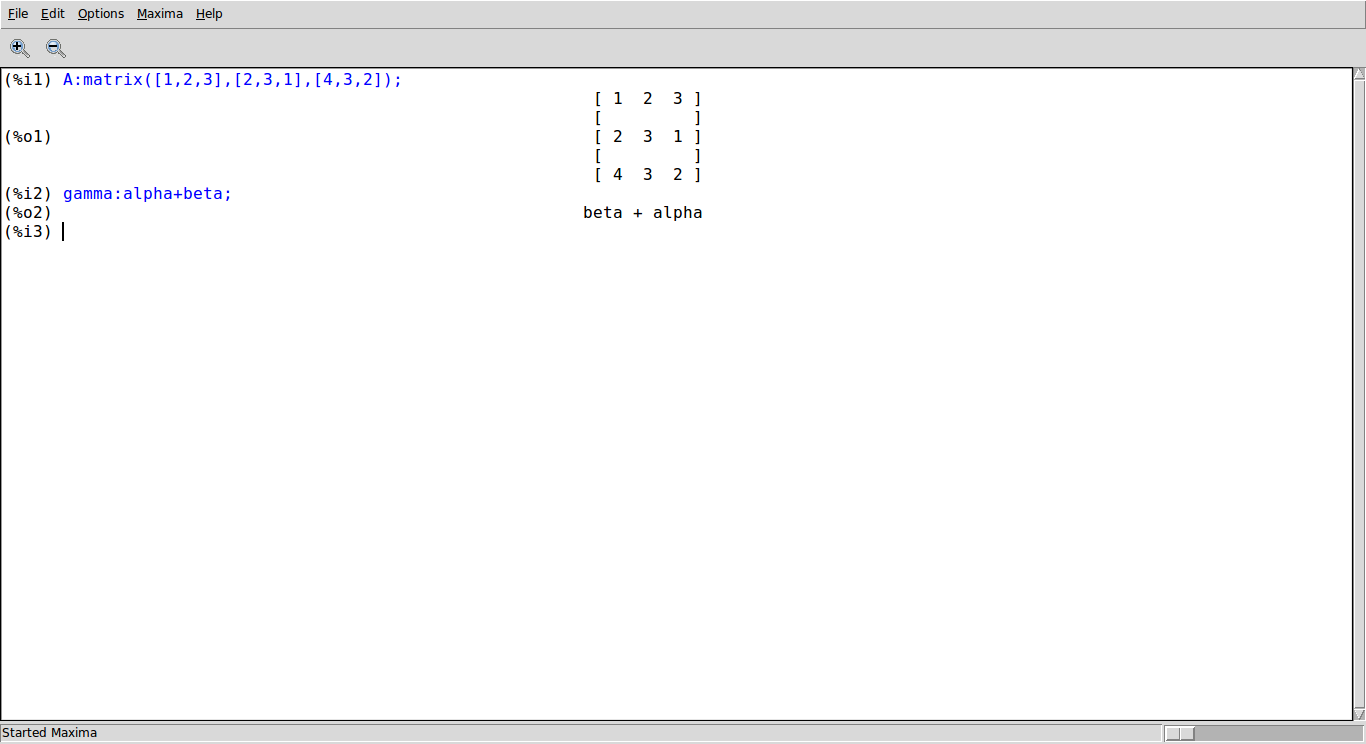
\includegraphics[width=\linewidth]
          {Figs/xmaxima}}
        \only<3,5>{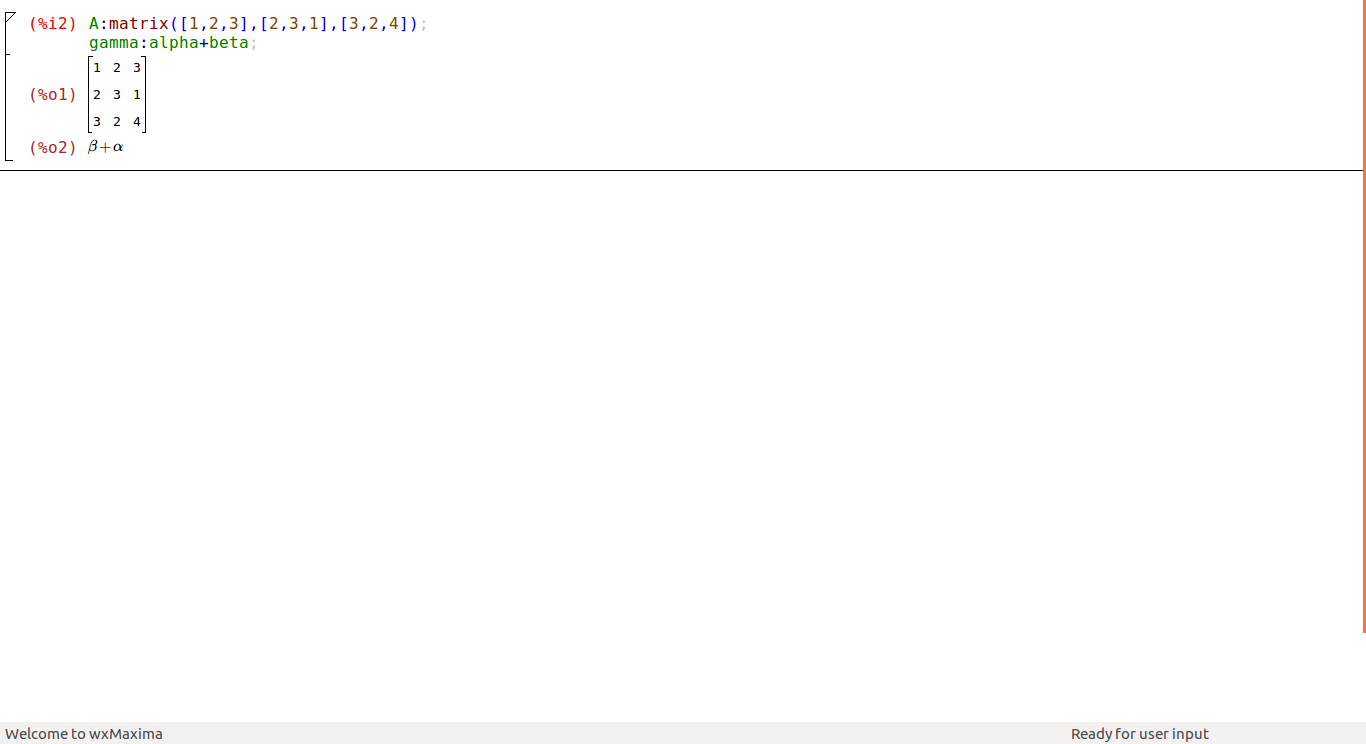
\includegraphics[width=\linewidth]
          {Figs/wxmaxima}}
        \only<4>{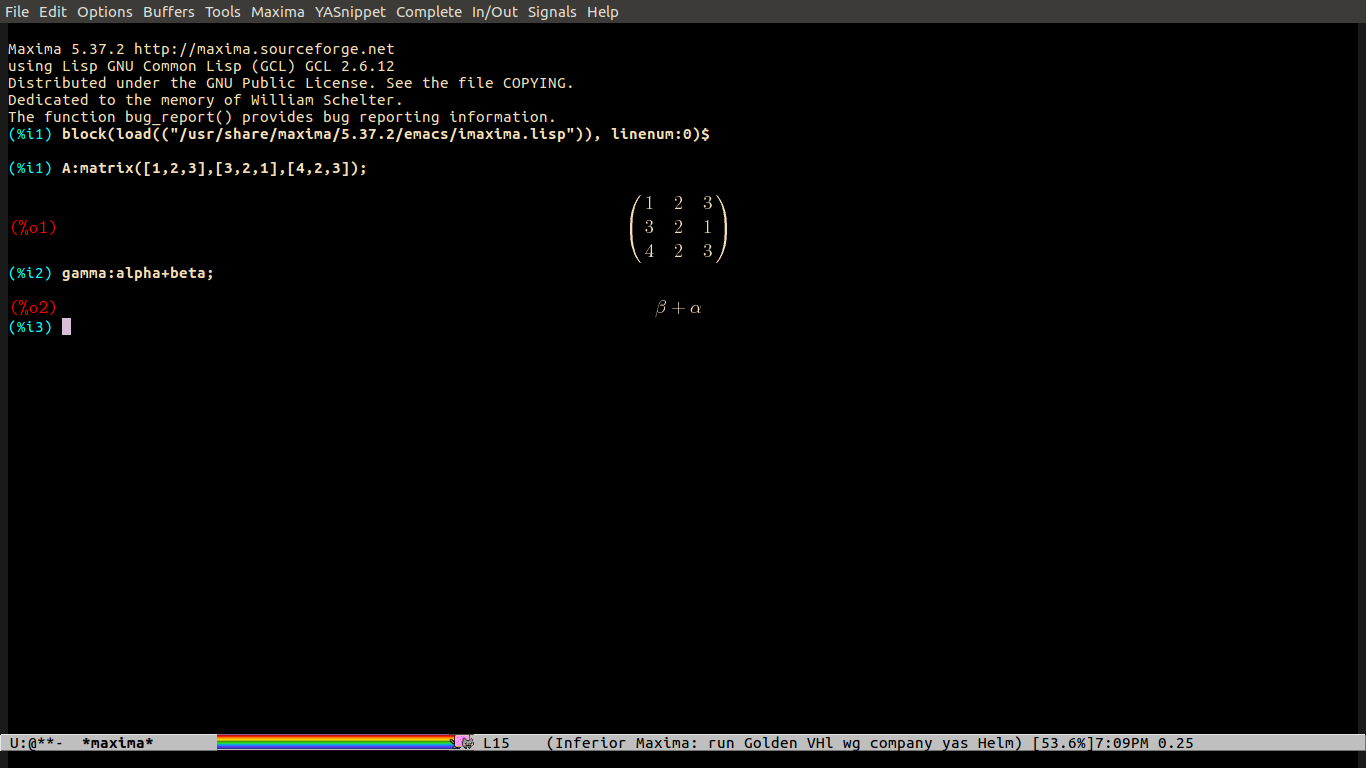
\includegraphics[width=\linewidth]
          {Figs/imaxima}}
      \end{center}
    \end{column}  
  \end{columns}
\end{frame}

\begin{frame}
  \frametitle{Maxima Init File}
  \begin{itemize}
  \item<.-> By default, the variable ``maxima_userdir'' stores the
    user directory (in Linux it is ~/.maxima'')
  \item<.-> You will have to create this directory and a file
    ``maxima-init.mac'' inside it
  \item<.-> Try adding ``disp(``Greetings!'')\$'' in the file and fire
    up maxima
  \end{itemize}
\end{frame}

\begin{frame}
  \frametitle{Command Summary}
  \begin{description}
  \item<.->[disp] display string to stdout
  \item<.->[describe,?] describe maxima command or variable
  \item<.->[apropos,??] inexact search for maxima command or variable
  \end{description}
\end{frame}

\section{Basics}

\begin{frame}[<1->]
  \frametitle{Some basics}
  \only<1>{\begin{itemize}
  \item Statements terminated by a ``;''
  \item Suppress output by terminating with a \$
  \item Variable assignment with ``:''
  \item Function declaration with ``:=''
  \item \alert{Note}: ``='' is a symbol, not an operator!
  \item Lists indices go as 1,2,3,...
  \item ``nouns'' and ``verbs''
  \end{itemize}}
  \only<2->{  \begin{columns}
    \begin{column}{.4\textwidth}
      \begin{maxima}
        diff(sin(x^2),x);
\maximaoutput*
\m  2\,x\,\cos x^2 \\
      \end{maxima}
    \end{column}
    \begin{column}{.6\textwidth}
      \begin{maxima}
        integrate(cos(x)*cosh(x),x);
        \maximaoutput*
        \m  {{e^ {- x }\,\left(\left(e^{2\,x}-1\right)\,\cos x+\left(e^{2\,x}+1\right)\,\sin x\right)}\over{4}} \\
      \end{maxima}
    \end{column}    
  \end{columns}}
\end{frame}

\begin{frame}[<1->]
  \frametitle{Basic Arithmetic}
  \textbf{Handling literals}
  \only<+>{
    \begin{columns}<.>
      \begin{column}<.>{0.5\textwidth}
        \begin{maxima}
          (1/2+sqrt(2/3))^2; \maximaoutput*
          \m  \left({{1}\over{2}}+{{\sqrt{2}}\over{\sqrt{3}}}\right)^2 \\
        \end{maxima}
      \end{column}
      \begin{column}<.>{0.5\textwidth}
        \begin{maxima}
          expand((1/2+sqrt(2/3))^2);
          \maximaoutput*
          \m  {{\sqrt{2}}\over{\sqrt{3}}}+{{11}\over{12}} \\
        \end{maxima}
      \end{column}
    \end{columns}
  }
  \only<+>{
    \begin{columns}<.>
      \begin{column}<.>{0.5\textwidth}
        \begin{maxima}
          expand((1/2+sqrt(2/3))^2), numer;          
\maximaoutput*
\m  1.733163247594392 \\
        \end{maxima}
      \end{column}
      \begin{column}<.>{0.5\textwidth}
        \begin{maxima}
          fpprec:20;
          bfloat(expand(
          (1/2+sqrt(2/3))^2));          
\maximaoutput*
\m  1\linebreak[0].\linebreak[0]7\linebreak[0]3\linebreak[0]3\linebreak[0]1\linebreak[0]6\linebreak[0]3\linebreak[0]2\linebreak[0]4\linebreak[0]7\linebreak[0]5\linebreak[0]9\linebreak[0]4\linebreak[0]3\linebreak[0]9\linebreak[0]2\linebreak[0]6\linebreak[0]9\linebreak[0]9\linebreak[0]4\linebreak[0]B\linebreak[0]0 \\
        \end{maxima}
      \end{column}
    \end{columns}
    }
\end{frame}

\begin{frame}[<1->]
  \frametitle{Algebra}
  \textbf{Handling Symbolics}
  \only<+>{
    \begin{columns}<.>
      \begin{column}<.>{0.5\textwidth}
        \begin{maxima}
          (x+3*y+x^2*y)^3; \maximaoutput*
          \m  \left(x+3\,y+x^2\,y\right)^3 \\
        \end{maxima}
      \end{column}
      \begin{column}<.>{0.5\textwidth}
        \begin{maxima}
          expand((x+3*y+x^2*y)^3); \maximaoutput*
          \m  x^6\,y^3+9\,x^4\,y^3+27\,x^2\,y^3+27\,y^3+3\,x^5\,y^2+18\,x^3\,y^2+27\,x\,y^2+3\,x^4\,y+9\,x^2\,y+x^3 \\
        \end{maxima}
      \end{column}
    \end{columns}
} 
  \only<+>{
    \begin{columns}<.>
      \begin{column}<.>{0.5\textwidth}
        \begin{maxima}
          expand(subst([x=5/y],
          (x+3*y+x^2*y)^3)); \maximaoutput*
          \m  27\,y^3+810\,y+{{8100}\over{y}}+{{27000}\over{y^3}} \\
        \end{maxima}
      \end{column}
      \begin{column}<.>{0.5\textwidth}
        \begin{maxima}
          factor(27*y^3+810*y+8100/y
          +2700/y^3); \maximaoutput*
          \m  {{27\,\left(100+300\,y^2+30\,y^4+y^6\right)}\over{y^3}} \\
        \end{maxima}
      \end{column}
    \end{columns}
}
  \only<+>{
    \begin{maxima}
      solve([expand(subst([x=5/y],(x+3*y+x^2*y)^3))=0],y);
\maximaoutput*
\m  \left[ y=-\sqrt{10}\,i , y=\sqrt{10}\,i \right] \\
    \end{maxima}
  }
  \only<+>{
    \begin{maxima}
      solve([x+y+z=4,y+z-2*x=5,z=4*x-3*y+t,t+y=z],[x,y,z,t]);
\maximaoutput*
\m  \left[ \left[ x=-{{1}\over{3}} , y=-{{1}\over{3}} , z={{14}\over{3}} , t=5 \right]  \right] \\
    \end{maxima}
  }
  \only<+>{
    \begin{columns}
      \begin{column}{0.5\textwidth}
        \begin{maxima}
          sum(1/n^2,n,0,N);
\maximaoutput*
\m  \sum_{n=0}^{N}{{{1}\over{n^2}}}\big. \\
        \end{maxima}
      \end{column}
      \begin{column}{0.5\textwidth}
        \begin{maxima}
          product(1/n^2,n,1,10);
\maximaoutput*
\m  {{1}\over{13168189440000}} \\
        \end{maxima}
      \end{column}      
    \end{columns}
  }  
\end{frame}

\begin{frame}
  \frametitle{Commands Summary}
  \begin{description}
  \item[diff]<1-> symbolic differentiation
  \item[integrate]<1-> symbolic integrations
  \item[numer]<1-> numerical result
  \item[fpprec]<1-> (variable) set floating point precision    
  \item[bfloat]<1-> floating point representation
  \item[expand]<1-> expand expression
  \item[factor]<1-> factor expression
  \item[subst]<1-> substitute for variables
  \item[solve]<1-> solve system
  \end{description}
\end{frame}

\section{Plotting}

\begin{frame}
  \frametitle{Plotting functions}
  \only<+>{
    \textbf{Explicit function plotting}
    \begin{maxima}
      plot2d(sin(x),[x,-\%pi,\%pi]);
      plot3d(sin(x+y)*cos(x-y),[x,-\%pi,\%pi],[y,-\%pi,\%pi]);
    \end{maxima}
    \textbf{pointer: try adding ``wx'' as a prefix in wxmaxima}
    \begin{figure}[h!]
      \centering
      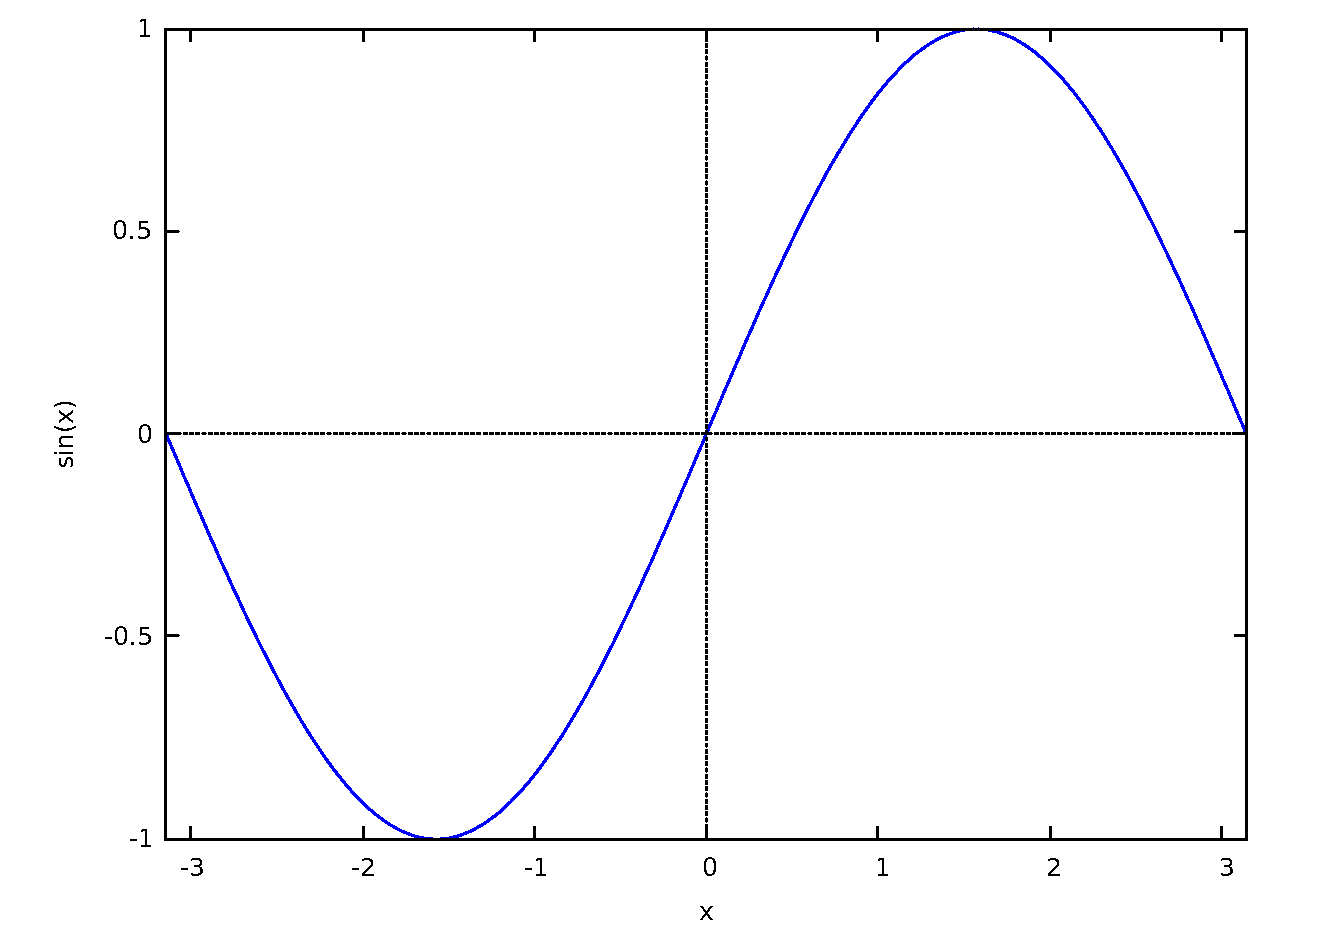
\includegraphics[width=0.5\linewidth]{Figs/plot2d}
      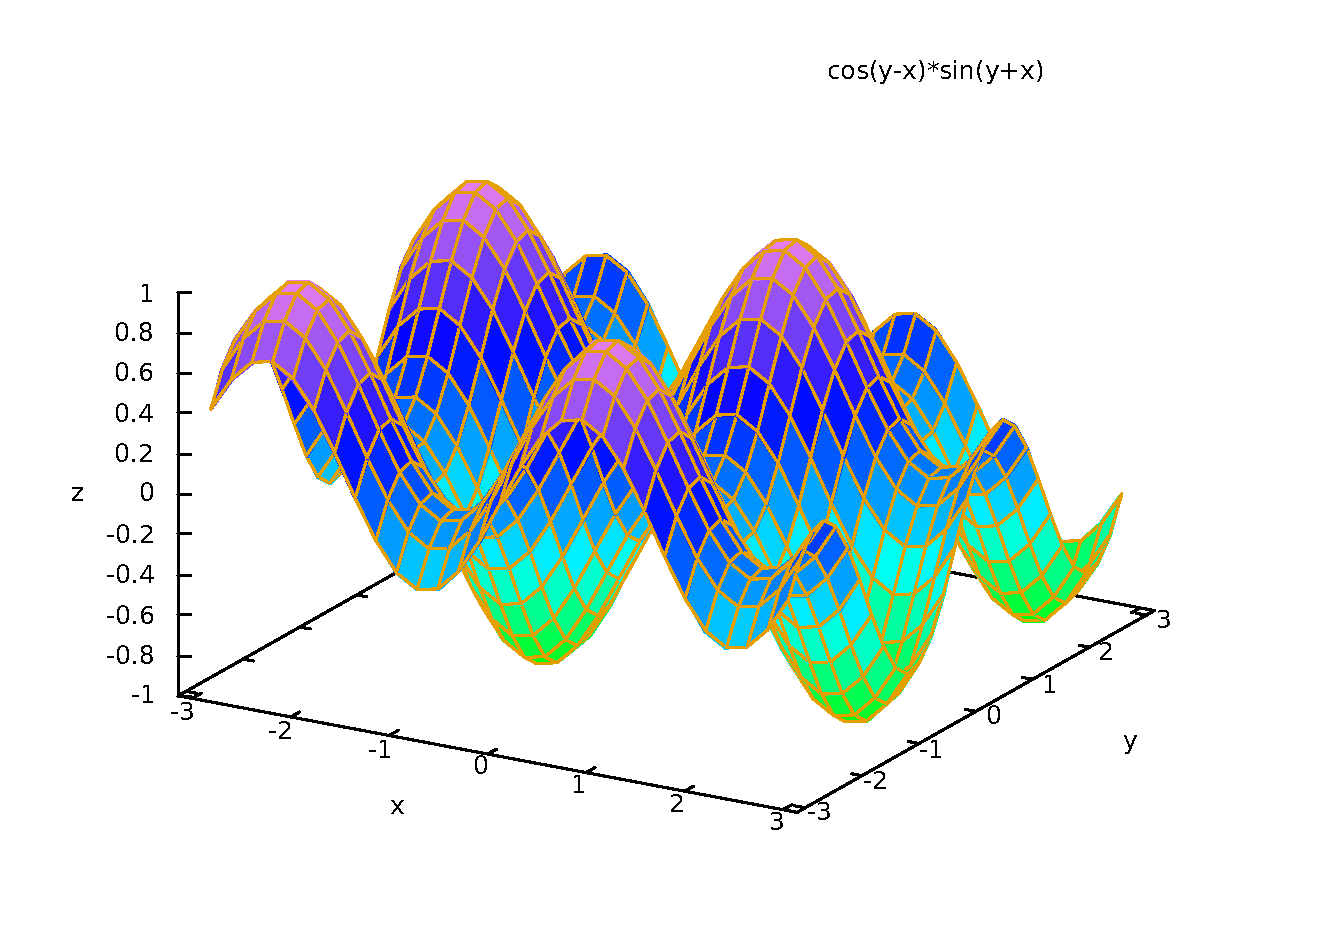
\includegraphics[width=0.5\linewidth]{Figs/plot3d}
    \end{figure}
  }
  \only<+>{
    \textbf{Implicit plots}
    \begin{maxima}
      load(implicit_plot);
      implicit_plot(x^2=y^2-3*y+1,[x,-4,4],[y,-4,4],
      [gnuplot_preamble,"set\ zeroaxis"]);
    \end{maxima}
    \vspace{-0.5cm}
    \begin{figure}[h!]
      \centering
      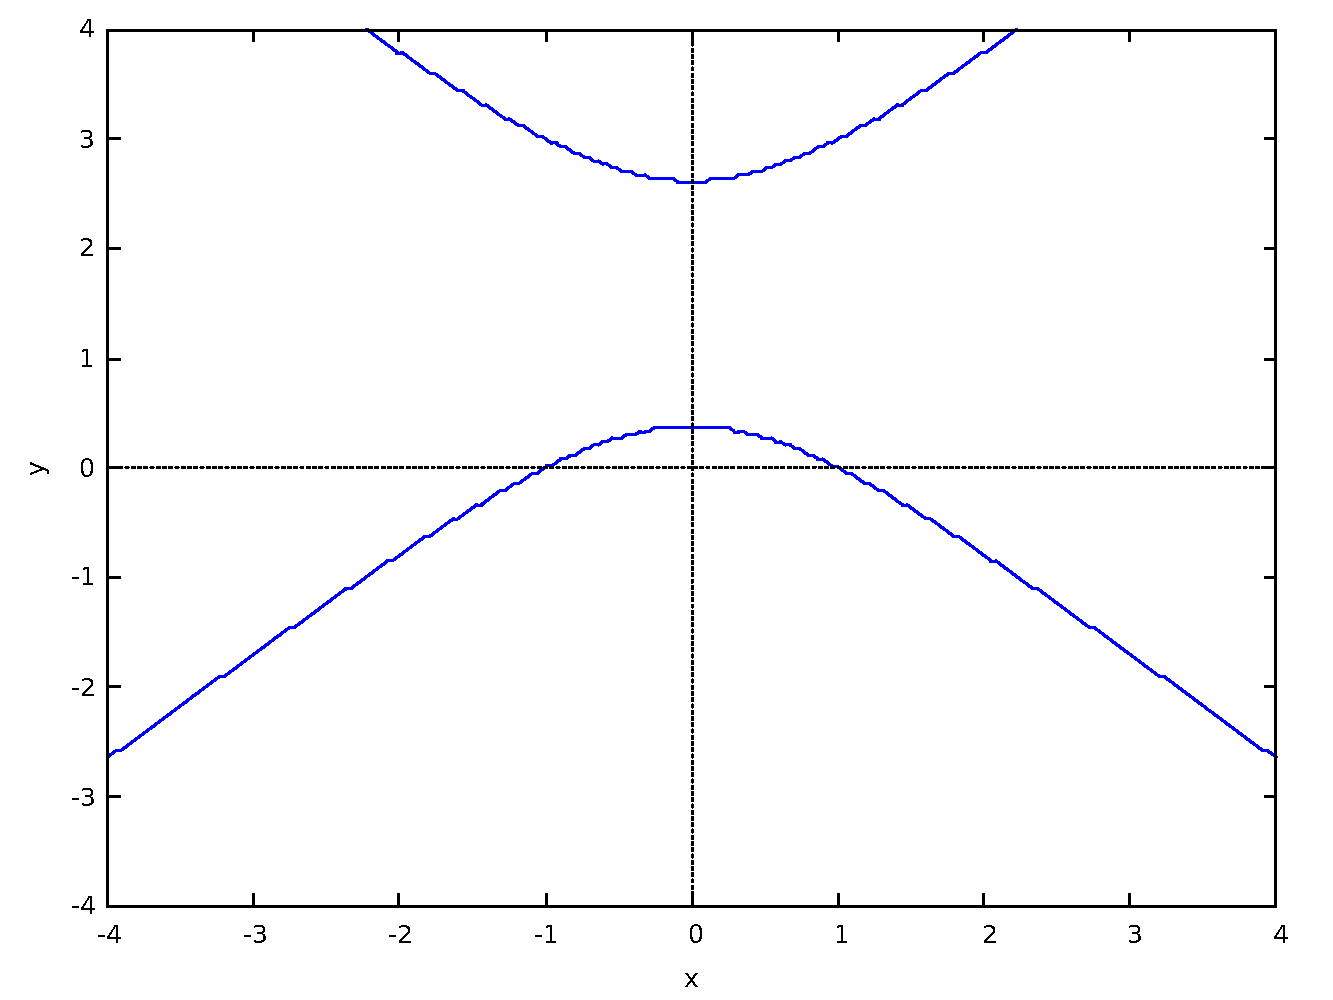
\includegraphics[width=0.5\linewidth]{Figs/implicit_plot}
    \end{figure}
  }
  \only<+>{
    \textbf{parametric plots}
    \begin{maxima}
      r(t):=t;
      plot2d([parametric,r(t)*cos(t),r(t)*sin(t), [t,-2*\%pi,2*\%pi],[nticks,80]],[x,-7,7]);
    \end{maxima}
    \vspace{-0.5cm}
    \begin{figure}[h!]
      \centering
      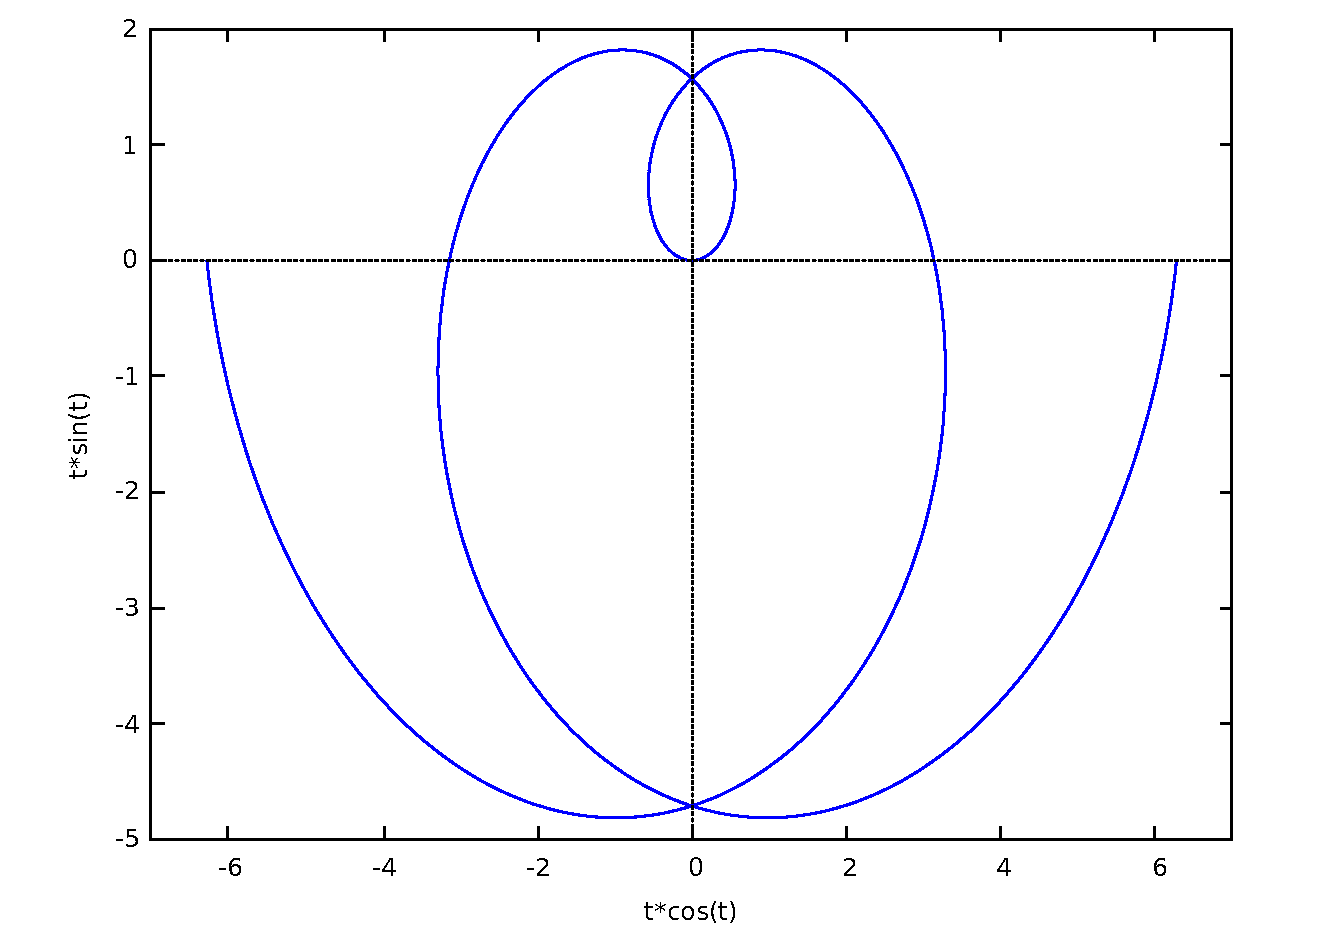
\includegraphics[width=0.5\linewidth]{Figs/2dparam}
    \end{figure}
  }
  \only<+>{
    \begin{maxima}
      expr_1:cos(y)*(12.0+6*cos(x));
      expr_2:sin(y)*(12.0+6*cos(x));
      expr_3:6*sin(x);
      plot3d([expr_1,expr_2,expr_3], [x,0,2*\%pi],[y,0,2*\%pi],[gnuplot_pm3d,true]);
    \end{maxima}
    \vspace{-0.8cm}
    \begin{figure}[h!]
      \centering
      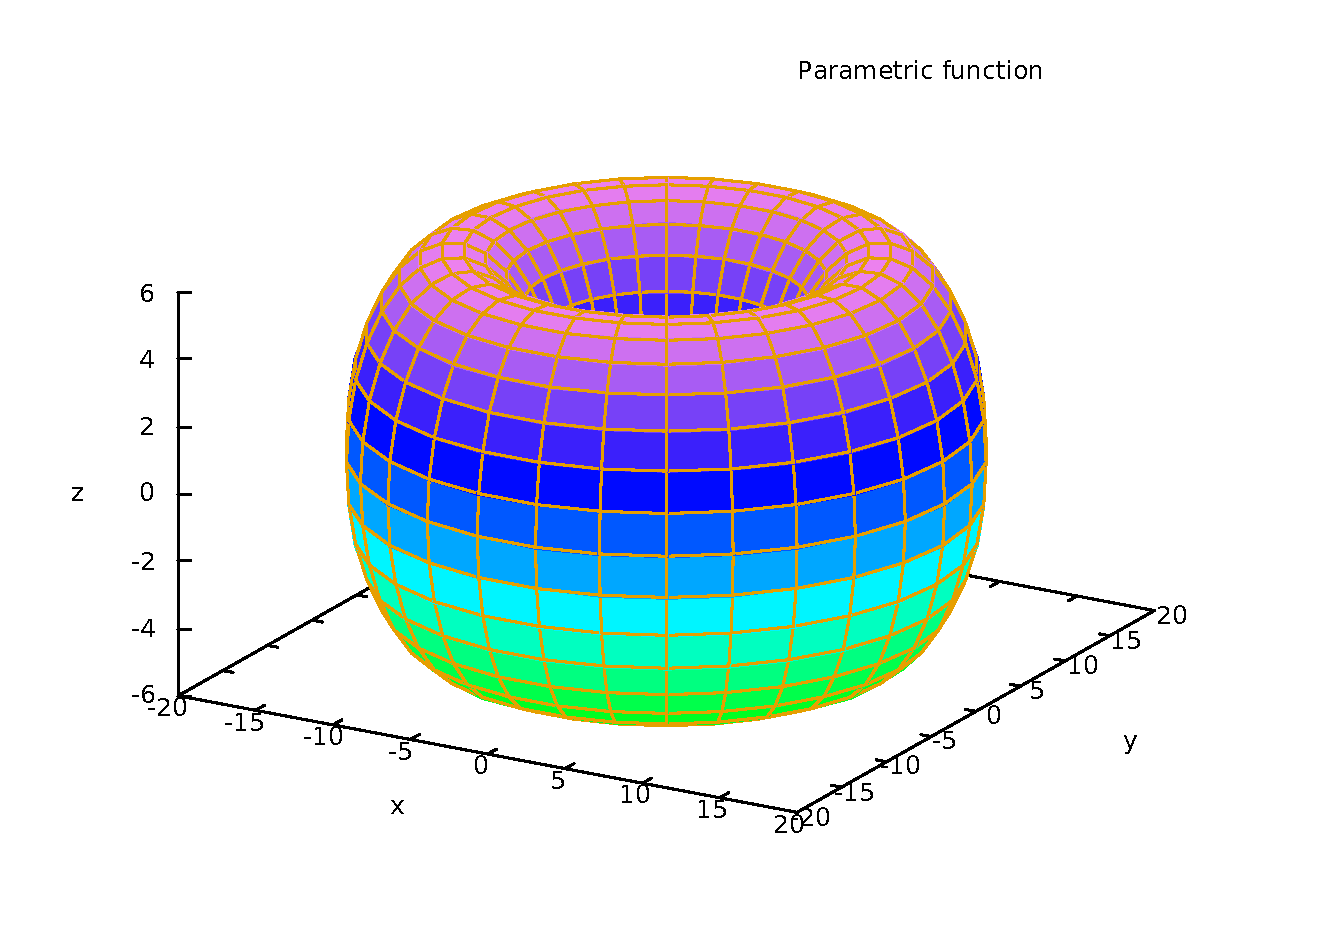
\includegraphics[width=0.5\linewidth]{Figs/torus}
    \end{figure}    
  }
  \only<+>{
    \textbf{Misc}
    \begin{maxima}
      set_plot_option([gnuplot_preamble,"set\ cntrparam levels\ 12"]);
      contour_plot(sin(y)*cos(x)^2,[x,-4,4],[y,-4,4]);
    \end{maxima}
    \vspace{-0.8cm}
    \begin{figure}[h!]
      \centering
      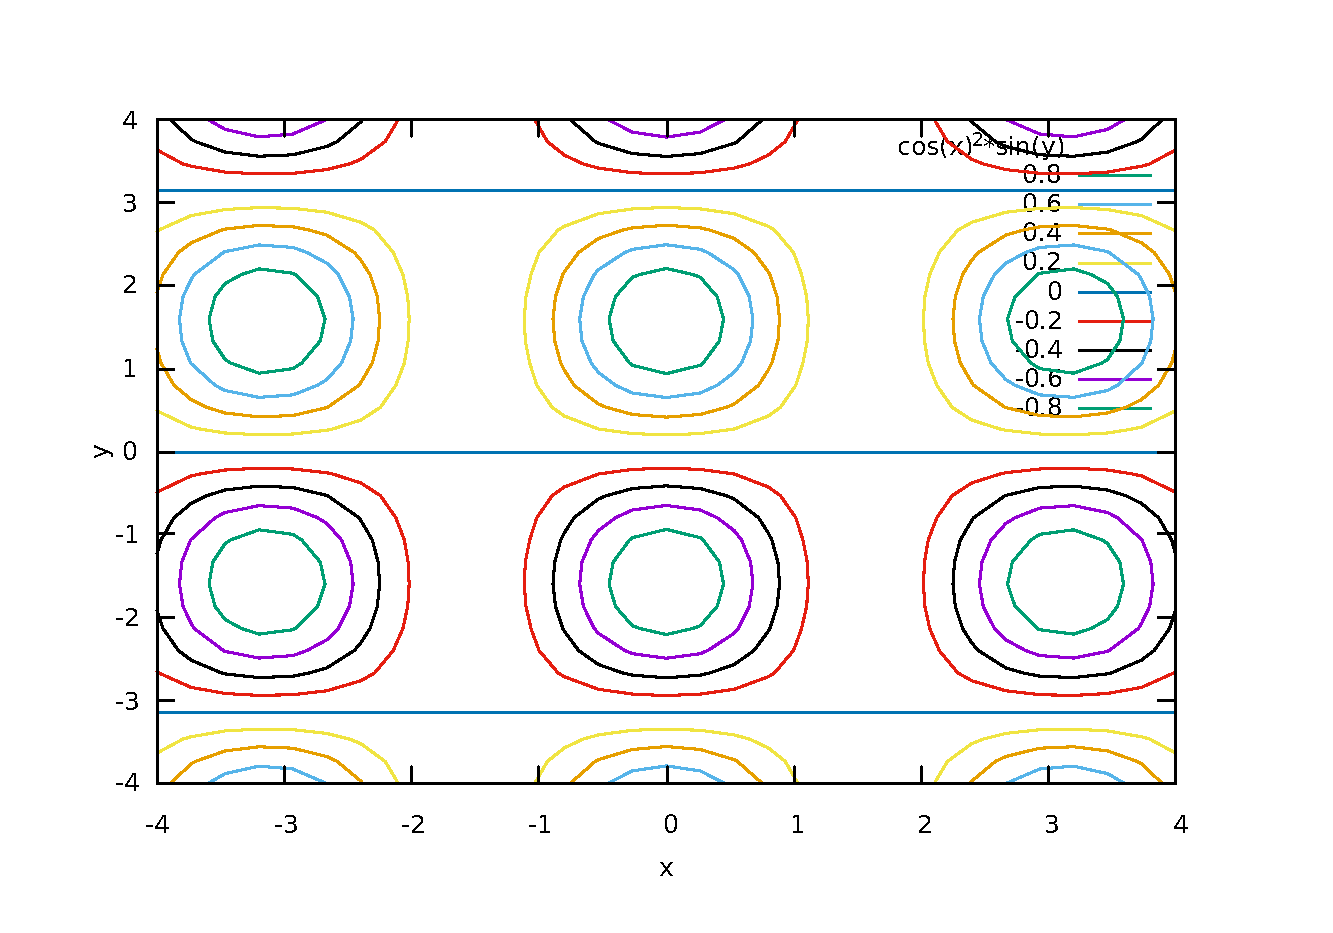
\includegraphics[width=0.5\linewidth]{Figs/cntr}
    \end{figure}        
  }
  \only<+>{
    \textbf{Discontinuous function}
    \begin{maxima}
      g(x):=\ if\ x>=1\ and\ x<2\ then\ (x-1)\ elseif\ x>=2 and\
      x<=3\ then\ (6-2*x)\ else\ 0;
\maximaoutput*
\m  g\left(x\right)\mathbin{:=}\mathbf{if}\;x\geq 1\land \left(x<2\right)\;\mathbf{then}\;x-1\;\mathbf{elseif}\;x\geq 2\land \left(x\leq 3\right)\;\mathbf{then}\;6-2\,x\;\mathbf{else}\;0 \\
    \end{maxima}
  }
  \only<+>{
    \begin{figure}
      \centering
      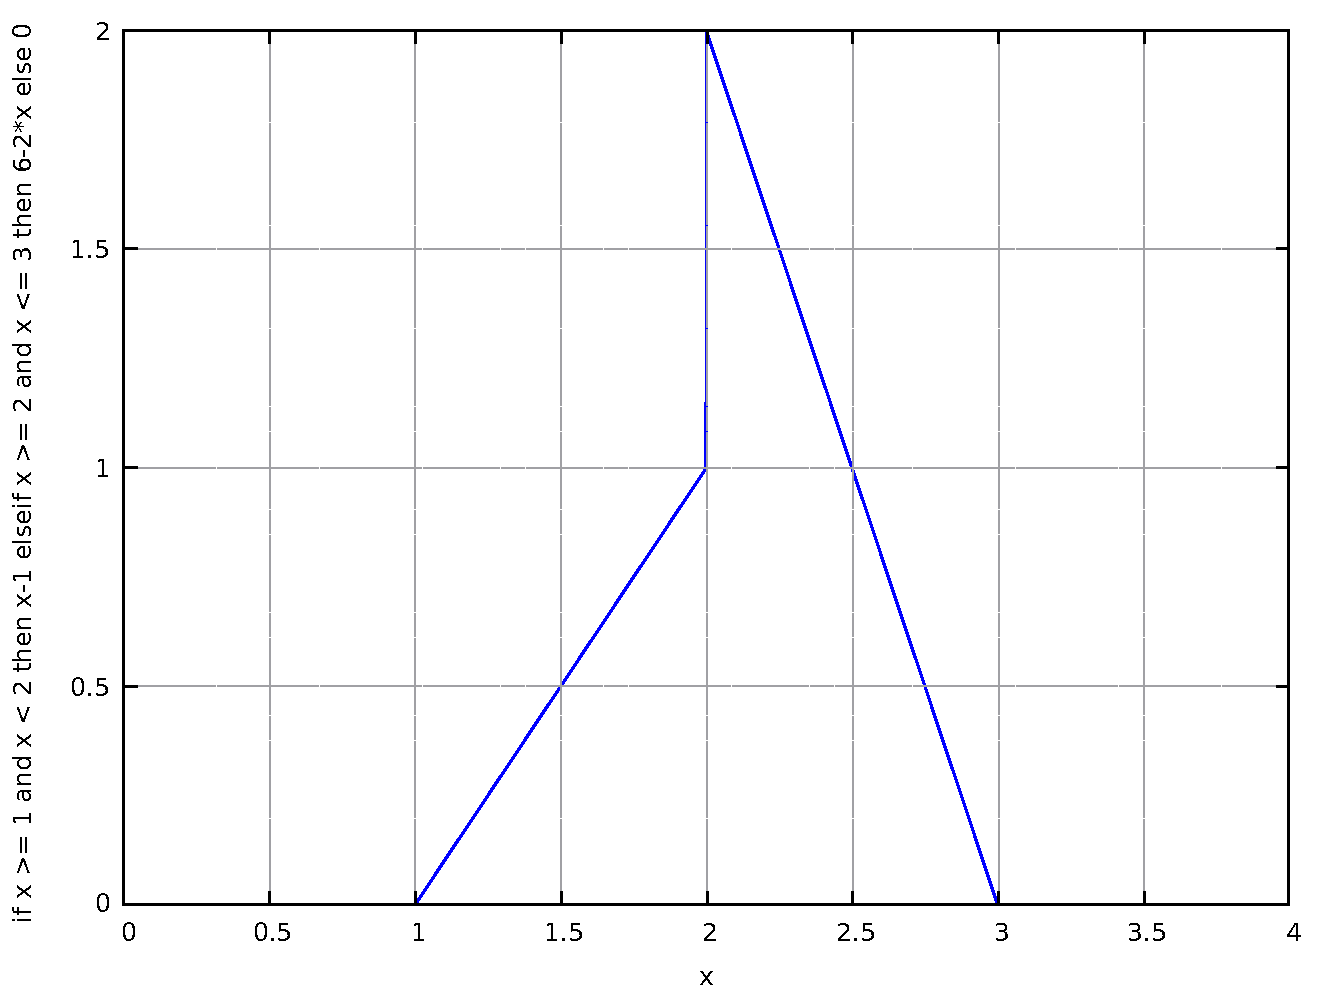
\includegraphics[width=0.6\linewidth]{Figs/discont}
    \end{figure}
  }
\end{frame}

\begin{frame}
  \frametitle{Commands Summary}
  \begin{description}
  \item<.->[plot2d] 2d plots
  \item<.->[plot3d] 3d plots
  \item<.->[implicit\_plot] plotting implicit expressions
  \item<.->[contour\_plot] contours
  \end{description}
\end{frame}

\section{Solving Equations}

\begin{frame}
  \frametitle{Systems of equations}
  \only<+>{
    \begin{maxima}
      apropos("solve");
\maximaoutput*
\m  \left[ \mathrm{baksolve} , \linebreak[0]\mathrm{desolve} , \linebreak[0]\mathrm{funcsolve} , \linebreak[0]\mathrm{globalsolve} , \linebreak[0]\mathrm{linsolve} , \linebreak[0]\mathrm{linsolvewarn} , \linebreak[0]\mathrm{linsolve\_by\_lu} , \linebreak[0]\mathrm{linsolve\_params} , \linebreak[0]\mathrm{solve} , \linebreak[0]\mathrm{solvedecomposes} , \linebreak[0]\mathrm{solveexplicit} , \linebreak[0]\mathrm{solvefactors} , \linebreak[0]\mathrm{solvenullwarn} , \linebreak[0]\mathrm{solveradcan} , \linebreak[0]\mathrm{solvetrigwarn} , \linebreak[0]\mathrm{tmlinsolve} \right] \\
    \end{maxima}
  }
  \only<+>{
    \textbf{linear systems}
    \begin{maxima}
      eq1:x+y=8*a*x-z+4*5;\
      eq2:y+z*\%pi=4*x;
      eq3:x-y+z=4;
      linsolve([eq1,eq2,eq3],[x,y,z]);
\maximaoutput*
\m  \left[ x=-\frac{8+12\,\pi}{\left(4+4\,\pi\right)\,a-\pi-4} , \linebreak[0]y=-\frac{32+8\,\pi+16\,\pi\,a}{\left(4+4\,\pi\right)\,a-\pi-4} , \linebreak[0]z=\frac{16\,a-40}{\left(4+4\,\pi\right)\,a-\pi-4} \right] \\
    \end{maxima}
  }
  \only<+>{
    \textbf{Algebraic Equation (analytic solution)}
    \begin{maxima}
      solve(a*x^2+b*x+c=0,x);
\maximaoutput*
\m  \left[ x=-\frac{b+\sqrt{b^2-4\,a\,c}}{2\,a} , \linebreak[0]x=\frac{\sqrt{b^2-4\,a\,c}-b}{2\,a} \right] \\
    \end{maxima}
  }
  \only<+>{
    \textbf{Substitute values}
    \begin{maxima}
      sol:solve(a*x^2+b*x+c=0,x);
      radcan(subst([a=1,b=2,c=3],sol[1]));
\maximaoutput*
\m  x=-\sqrt{2}\,i-1 \\
    \end{maxima}
  }  
  \only<+>{
    \textbf{System of algebraic equations}
    \begin{maxima}
      f(x):=x^2-1;
      solve([f(x/y)=0,f(x*y)=0],[x,y]);
\maximaoutput*
\m  f\left(x\right)\mathbin{:=}x^2-1 \\
\m  \left[ \left[ x=-1 , \linebreak[0]y=1 \right]  , \linebreak[0]\left[ x=1 , \linebreak[0]y=-1 \right]  , \linebreak[0]\left[ x=-i , \linebreak[0]y=-i \right]  , \linebreak[0]\left[ x=i , \linebreak[0]y=i \right]  , \linebreak[0]\left[ x=-i , \linebreak[0]y=i \right]  , \linebreak[0]\left[ x=i , \linebreak[0]y=-i \right]  , \linebreak[0]\left[ x=-1 , \linebreak[0]y=-1 \right]  , \linebreak[0]\left[ x=1 , \linebreak[0]y=1 \right]  \right] \\
    \end{maxima}
  }
  \only<+>{
    \textbf{Polynomials \& Numerical solutions}
    \begin{maxima}
      allroots(x^5+x^2-x+8=0);          
\maximaoutput*
\m  \left[ x=0.9189543576112322\,i+1.179427901164746 , \linebreak[0]x=1.179427901164746-0.9189543576112322\,i , \linebreak[0]x=1.427958893635229\,i-0.3522627040736663 , \linebreak[0]x=-1.427958893635229\,i-0.3522627040736663 , \linebreak[0]x=-1.65433039418216 \right] \\
    \end{maxima}
  }
  \only<+>{
    \textbf{Checking Solution}
    \begin{maxima}
      f(x):=x^3+x^2-x+8$\
      sol:allroots(f(x))$
      expand(map(f,sol));
\maximaoutput*
\m  \left[ x^3+x^2-x+8=4.440892098500626 \times 10^{-16}\,i+1.77635683940025 \times 10^{-15} , \linebreak[0]x^3+x^2-x+8=1.77635683940025 \times 10^{-15}-4.440892098500626 \times 10^{-16}\,i , \linebreak[0]x^3+x^2-x+8=0.0 \right] \\
    \end{maxima}
  }
  \only<+>{
    \begin{columns}<.>
      \begin{column}<.>{0.5\textwidth}
        \begin{maxima}
          load(newton);
          newton(x^7-5*x^6+4*x^4- 5*x^2+x+2,0);
\maximaoutput*
\m  -5.763042928902195_B \times 10^{-1} \\
        \end{maxima}
      \end{column}
      \begin{column}<.>{0.5\textwidth}
        \begin{maxima}
          newton(x^7-5*x^6+4*x^4- 5*x^2+x+2,1);
\maximaoutput*
\m  8.194213634964119_B \times 10^{-1} \\
        \end{maxima}
      \end{column}      
    \end{columns}
  }
\end{frame}

\begin{frame}
  \frametitle{Commands Summary}
  \begin{description}
  \item<1->[apropos] apropos search
  \item<1->[linsolve] solve linear systems
  \item<1->[solve] solve algebraic equations
  \item<1->[subst] substitute values to expressions
  \item<1->[allroots] numerically estimate all roots of a polynomial
  \item<1->[kill] ``kill(a,b,c);'' lets you delete unwanted variables
  \item<1->[map] map the solutions to a function
  \end{description}
\end{frame}

\section{Vectors and Matrices}

\subsection{Vectors}
\begin{frame}
  \frametitle{Vectors}
  \only<+>{  \begin{maxima}
    load(vector);
    functions;
\maximaoutput*
\m  \left[ \mathrm{dimension}\left(\right) , \linebreak[0]\mathrm{type}\left(\mathrm{arg}\right) , \linebreak[0]\mathrm{coordsystem}\left(\mathrm{sys}\right) , \linebreak[0]\mathrm{cross}\left(a , \linebreak[0]b\right) , \linebreak[0]\mathrm{grad}\left(s\right) , \linebreak[0]\mathrm{div}\left(v\right) , \linebreak[0]\mathrm{curl}\left(a\right) , \linebreak[0]\mathrm{laplacian}\left(a\right) , \linebreak[0]\mathrm{dotdel}\left(v , \linebreak[0]b\right) , \linebreak[0]\mathrm{christoffel}\left(\right) , \linebreak[0]\mathrm{curlgrad}\left(s\right) , \linebreak[0]\mathrm{graddiv}\left(v\right) , \linebreak[0]\mathrm{divcurl}\left(v\right) \right] \\
\end{maxima}}
\only<+>{
  \begin{columns}<.>
    \begin{column}<.>{0.5\textwidth}
      \begin{maxima}
        v1:[x1,y1,z1]$
        v2:[x2,y2,z2]$
        v1\ cross\ v2;
\maximaoutput*
\m  \left[ \mathrm{y1}\,\mathrm{z2}-\mathrm{y2}\,\mathrm{z1} , \linebreak[0]\mathrm{x2}\,\mathrm{z1}-\mathrm{x1}\,\mathrm{z2} , \linebreak[0]\mathrm{x1}\,\mathrm{y2}-\mathrm{x2}\,\mathrm{y1} \right] \\
      \end{maxima}
    \end{column}
    \begin{column}<.>{0.5\textwidth}
      \begin{maxima}
        v1.v2;
\maximaoutput*
\m  \mathrm{z1}\,\mathrm{z2}+\mathrm{y1}\,\mathrm{y2}+\mathrm{x1}\,\mathrm{x2} \\
      \end{maxima}
    \end{column}
  \end{columns}
}
\end{frame}

\subsection{Matrices and Linear Algebra}

\begin{frame}
  \frametitle{Matrices and Linear Algebra}
  \only<+>{
    \begin{maxima}
      load(diag);
      A:matrix([a,b,c],[d,e,f],[g,h,i]);
      col(A,1);
      row(A,2);
      invert(A);
      transpose(A);
      determinant(A);
      list_matrix_entries(A);      
    \end{maxima}
    \textbf{Row major!}
  }
  \only<+>{
    \textbf{Matrix Products}
    \begin{maxima}
      load(diag);
      A:matrix([a,b,c],[d,e,f],[g,h,i]);      
      B:transpose(matrix([c,d,e]));
      A.B;
      A*A;
      A^2;
      A^^2;
      rank(A);      
    \end{maxima}
  }
  \only<+>{
    \textbf{Matrix properties}
    \begin{maxima}
      A:matrix([1,2],[4,5]);
      eigenvectors(A);
\maximaoutput*
\m  \left[ \left[ \left[ 3-2\,\sqrt{3} , \linebreak[0]2\,\sqrt{3}+3 \right]  , \linebreak[0]\left[ 1 , \linebreak[0]1 \right]  \right]  , \linebreak[0]\left[ \left[ \left[ 1 , \linebreak[0]1-\sqrt{3} \right]  \right]  , \linebreak[0]\left[ \left[ 1 , \linebreak[0]\sqrt{3}+1 \right]  \right]  \right]  \right] \\
    \end{maxima}
  }
  \only<+>{
    \textbf{Other functionality}
    \begin{maxima}
      load(eigen);
      load(linearalgebra);
    \end{maxima}
  }
\end{frame}

\begin{frame}
  \frametitle{Command Summary}
  \begin{description}
  \item<.->[matrix] create a matrix
  \item<.->[col] access column of a matrix
  \item<.->[row] access row of a matrix
  \item<.->[transpose] transpose of a matrix
  \item<.->[determinant] obtain the determinant of a matrix
  \item<.->[rank] obtain the rank of a matrix    
  \item<.->[invert] invert a matrix
  \item<.->[list\_matrix\_entries] list out the matrix in row major
  \item<.->[eigenvectors] obtain the eigen vectors
  \end{description}
\end{frame}

\section{Calculus}

\subsection{Differential Calculus}

\begin{frame}
  \frametitle{Differential Calculus}
  \only<+>{
    \begin{columns}<.>
      \begin{column}<.>{0.5\linewidth}
        \textbf{Independant variable specified}
        \begin{maxima}
          diff(x^n,x,2);
\maximaoutput*
\m  \left(n-1\right)\,n\,x^{n-2} \\
        \end{maxima}
      \end{column}      
      \begin{column}<.>{0.5\linewidth}
        \textbf{Unspecified independant variable}        
        \begin{maxima}
          diff(x^n);
\maximaoutput*
\m  n\,x^{n-1}\,dx+x^{n}\,\log x\,dn \\
        \end{maxima}
      \end{column}
    \end{columns}
  }
  \only<+>{
    $$\mathbf{\frac{\partial}{\partial y}\frac{\partial^2}{\partial x^2}}\left(\sin(x)\cos(y-x)\right)$$
    \begin{maxima}
      diff(sin(x)*cos(y-x),x,2,y,1);
\maximaoutput*
\m  2\,\sin x\,\sin \left(y-x\right)+2\,\cos x\,\cos \left(y-x\right) \\
    \end{maxima}
  }
  \only<+>{
    \begin{maxima}
      declare(a,constant);
      depends([x,y],t);
      diff(x^2+a*y^2,t);
      \maximaoutput*
      \m  2\,a\,y\,\left({{d\,y}\over{d\,t}}\right)+2\,x\,\left({{d\,x}\over{d\,t}}\right) \\
    \end{maxima}
    \textbf{Try out ``properties(a);'' \& ``propvars(constant);''}
  }
  \only<+>{
    \begin{columns}<.>
      \begin{column}<.>{0.5\linewidth}
        \begin{maxima}
          gp:diff(x^(2/3),x); limit(gp,x,0,plus);
\maximaoutput*
\m  {{2}\over{3\,x^{{{1}\over{3}}}}} \\
\m  \infty \\
        \end{maxima}
      \end{column}
      \begin{column}<.>{0.5\linewidth}
        \begin{maxima}
          limit(gp,x,0,minus); limit(gp,x,0);
\maximaoutput*
\m  -\infty \\
\m  \mathrm{infinity} \\
        \end{maxima}
      \end{column}
    \end{columns}
  }
  \only<+>{
    \begin{columns}<.>
      \begin{column}<.>{0.5\linewidth}
        \begin{maxima}
          dydx(expr,x,y):= diff(expr,x)/diff(expr,y);
\maximaoutput*
\m  \mathrm{dydx}\left(\mathrm{expr} , x , y\right)\mathbin{:=}{{\mathrm{diff}\left(\mathrm{expr} , x\right)}\over{\mathrm{diff}\left(\mathrm{expr} , y\right)}} \\
        \end{maxima}
      \end{column}
      \begin{column}<.>{0.5\linewidth}
        \begin{maxima}
          dydx(cos(x^2-y^2),x,y);
\maximaoutput*
\m  -{{x}\over{y}} \\
        \end{maxima}
      \end{column}
    \end{columns}
  }
\end{frame}

\subsection{Taylor Series}
\begin{frame}
  \frametitle{Taylor (or Laurent) series}
  \only<+>{
    \begin{maxima}
      taylor(f(x),x,0,3);
\maximaoutput*
\m  f\left(0\right)+\left(\left.{{d\,f\left(x\right)}\over{d\,x}}\right|_{x=0}\right)\,x+{{\left(\left.{{d^2\,f\left(x\right)}\over{d\,x^2}}\right|_{x=0}\right)\,x^2}\over{2}}+{{\left(\left.{{d^3\,f\left(x\right)}\over{d\,x^3}}\right|_{x=0}\right)\,x^3}\over{6}}+\cdots \\
    \end{maxima}
  }
  \only<+>{
    \begin{maxima}
      taylor(cos(x),x,0,10);
      taylor(sin(x),x,0,10);      
\maximaoutput*
\m  1-{{x^2}\over{2}}+{{x^4}\over{24}}-{{x^6}\over{720}}+{{x^8}\over{40320}}-{{x^{10}}\over{3628800}}+\cdots \\
\m  x-{{x^3}\over{6}}+{{x^5}\over{120}}-{{x^7}\over{5040}}+{{x^9}\over{362880}}+\cdots \\
    \end{maxima}
  }
  \only<+>{
    \begin{maxima}
      taylor(cos(x+y),[x,y],[0,0],[2,4]);
      factor(ratsimp(\%));
\maximaoutput*
\m  1-{{y^2+2\,y\,x+x^2}\over{2}}+{{y^4+4\,y^3\,x+6\,y^2\,x^2+4\,y\,x^3+x^4}\over{24}}+\cdots \\
\m  {{24-12\,x^2+x^4-24\,x\,y+4\,x^3\,y-12\,y^2+6\,x^2\,y^2+4\,x\,y^3+y^4}\over{24}} \\
    \end{maxima}
  }
  \only<+>{
    \begin{maxima}
      taylor(sin(x+y),[x,0,4],[y,0,4]);
\maximaoutput*
\m  y-{{y^3}\over{6}}+\cdots +\left({{y^4}\over{24}}-{{y^2}\over{2}}+1+\cdots \right)\,x+\left({{y^3}\over{12}}-{{y}\over{2}}+\cdots \right)\,x^2+\left(-{{y^4}\over{144}}+{{y^2}\over{12}}-{{1}\over{6}}+\cdots \right)\,x^3+\left(-{{y^3}\over{144}}+{{y}\over{24}}+\cdots \right)\,x^4+\cdots \\
    \end{maxima}
  }  
\end{frame}

\subsection{Symbolic Integration}

\begin{frame}
  \frametitle{Symbolic Integration}
  \only<+>{
    \begin{columns}<.>
      \begin{column}<.>{0.5\textwidth}
        \begin{maxima}
          integrate(f(x),x);
\maximaoutput*
\m  \int {f\left(x\right)}{\;dx}\big. \\
        \end{maxima}
      \end{column}
      \begin{column}<.>{0.5\textwidth}
        \begin{maxima}
          trigsimp(trigreduce
          (integrate(sin(x)^3,x)));
\maximaoutput*
\m  \frac{\cos \left(3\,x\right)-9\,\cos x}{12} \\
        \end{maxima}
      \end{column}      
    \end{columns}
  }
  \only<+>{
    \begin{columns}<.>
      \begin{column}<.>{0.5\textwidth}
        \begin{maxima}
          integrate(x^2*exp(-x^2),x);
\maximaoutput*
\m  \frac{\sqrt{\pi}\,\mathrm{erf}\left(x\right)}{4}-\frac{x\,e^ {- x^2 }}{2} \\
        \end{maxima}
      \end{column}
      \begin{column}<.>{0.5\textwidth}
        \begin{maxima}
          float(integrate( x^2*exp(-x^2),x,1,2));
\maximaoutput*
\m  0.2332527106719843 \\
        \end{maxima}
      \end{column}      
    \end{columns}
  }
  \only<+>{
    \begin{columns}<.>
      \begin{column}<.>{0.5\textwidth}
        \begin{maxima}
          expr:'integrate (2*x*(x^2+1)^3,x);
\maximaoutput*
\m  2\,\int {x\,\left(1+x^2\right)^3}{\;dx}\big. \\
\end{maxima}
\end{column}
      \begin{column}<.>{0.5\textwidth}
        \begin{maxima}
          exprc:changevar (expr,x^2+1-u,u,x);
\maximaoutput*
\m  \int {u^3}{\;du}\big. \\
        \end{maxima}        
      \end{column}
    \end{columns}
  }
  \only<+>{
    \begin{columns}<.>
      \begin{column}<.>{0.5\textwidth}
        \begin{maxima}
          ev(exprc,nouns); \maximaoutput*
          \m  \frac{u^4}{4} \\
        \end{maxima}
      \end{column}
      \begin{column}<.>{0.5\textwidth}
        \begin{maxima}
          subst([u=x^2+1], ev(exprc,nouns)); 
\maximaoutput*
\m  \frac{\left(1+x^2\right)^4}{4} \\
        \end{maxima}
      \end{column}      
    \end{columns}
  }  
\end{frame}

\begin{frame}
  \frametitle{Command Summary }
  \begin{description}
  \item<.->[diff] differentiate expression
  \item<.->[grind] ``non-pretty'' output
  \item<.->[display2d] set to true for pretty output
  \item<.->[declare] declare a symbol as constant
  \item<.->[depends] establish dependency
  \item<.->[integrate] integrate expression
  \item<.->[changevar] apply a change of variable
  \end{description}
\end{frame}

\section{Symbolic Manipulations}

\begin{frame}
  \frametitle{Simplifying Expressions}
  \only<+>{
    \textbf{factoring and expanding polynomials}
    \begin{columns}<.>
      \begin{column}<.>{0.5\textwidth}
        \begin{maxima}
          factor(x^2+2*x+1);
\maximaoutput*
\m  \left(1+x\right)^2 \\
        \end{maxima}
      \end{column}
      \begin{column}<.>{0.5\textwidth}
        \begin{maxima}
          expand((x+1)**2);
\maximaoutput*
\m  x^2+2\,x+1 \\
        \end{maxima}
      \end{column}      
    \end{columns}
  }
  \only<+>{
    \textbf{Trigonometric expressions}
    \begin{columns}<.>
      \begin{column}<.>{0.5\textwidth}
        \begin{maxima}
          trigsimp(sin(x)^2 +cos(x)^2);
\maximaoutput*
\m  1 \\
        \end{maxima}
      \end{column}
      \begin{column}<.>{0.5\textwidth}
        \begin{maxima}
          trigexpand(cos(x+3*y));
\maximaoutput*
\m  \cos x\,\cos \left(3\,y\right)-\sin x\,\sin \left(3\,y\right) \\
        \end{maxima}
      \end{column}      
    \end{columns}
  }
  \only<+>{
    \textbf{Rational expressions}
    \begin{columns}<.>
      \begin{column}<.>{0.5\textwidth}
        \begin{maxima}
          ratsimp((x^2+2*x+1)/ (x+1)+1/(4*x+3));
\maximaoutput*
\m  {{4+7\,x+4\,x^2}\over{4\,x+3}} \\
        \end{maxima}
      \end{column}
      \begin{column}<.>{0.5\textwidth}
        \begin{maxima}
          ratexpand((x^2+2*x+1)/ (x+1)+1/(4*x+3)); 
\maximaoutput*
\m  {{4\,x^2}\over{4\,x+3}}+{{7\,x}\over{4\,x+3}}+{{4}\over{4\,x+3}} \\
        \end{maxima}
      \end{column}      
    \end{columns}
  }
  \only<+>{
    \textbf{Complex exponentials}
    \begin{columns}<.>
      \begin{column}<.>{0.5\textwidth}
        \begin{maxima}
          demoivre:true;
          exp(a+b*\%i);
\maximaoutput*
\m  e^{a}\,\left(i\,\sin b+\cos b\right) \\
        \end{maxima}
      \end{column}
      \begin{column}<.>{0.5\textwidth}
        \begin{maxima}
          demoivre:false;
          exp(a+b*\%i);
\maximaoutput*
\m  e^{a+i\,b} \\
        \end{maxima}
      \end{column}      
    \end{columns}
  }
  \only<+>{
    \textbf{expand(expr,p,n);}
    \begin{columns}<.>
      \begin{column}<.>{0.5\textwidth}
        \begin{maxima}
          expand((x+1)^5+(x+1)^(-5) ,3,5);
\maximaoutput*
\m  {{1}\over{x^5+5\,x^4+10\,x^3+10\,x^2+5\,x+1}}+\left(1+x\right)^5 \\
        \end{maxima}
      \end{column}
      \begin{column}<.>{0.5\textwidth}
        \begin{maxima}
          expand((x+1)^5+(x+1)^(-5) ,5,3);
\maximaoutput*
\m  {{1}\over{\left(1+x\right)^5}}+x^5+5\,x^4+10\,x^3+10\,x^2+5\,x+1 \\
        \end{maxima}
      \end{column}      
    \end{columns}
  }
  \only<+>{
    \textbf{Partial fractions}        
    \begin{maxima}
      partfrac(1/(x^2+3*x+2),x);
      \maximaoutput*
      \m  {{1}\over{x+1}}-{{1}\over{x+2}} \\
    \end{maxima}
  }  
  \only<+>{
    \textbf{Expressions with logs, exponentials and radicals}
    \begin{columns}<.>
      \begin{column}<.>{0.5\textwidth}
        \begin{maxima}
          radcan((log(x+x^2)- log(x))^a/log(1+x)^(a/2));
\maximaoutput*
\m  \left(\log \left(1+x\right)\right)^{{{a}\over{2}}} \\
        \end{maxima}
      \end{column}
      \begin{column}<.>{0.5\textwidth}
        \begin{maxima}
          radcan((\%e^x-1)/ (1+\%e^(x/2)));
\maximaoutput*
\m  e^{{{x}\over{2}}}-1 \\
        \end{maxima}
      \end{column}      
    \end{columns}
  }
  \only<+>{
    \begin{columns}<.>
      \begin{column}<.>{0.5\textwidth}
        \begin{maxima}
          expr:sin(x^2+y^2)-sin(3*x);
          eq1:x^2+y^2-x=0;
\maximaoutput*
\m  \sin \left(x^2+y^2\right)-\sin \left(3\,x\right) \\
\m  y^2+x^2-x=0 \\
        \end{maxima}
      \end{column}
      \begin{column}<.>{0.5\textwidth}
        \textbf{Simplification with rules}        
        \begin{maxima}
          eq2:sin(x)=y;
          scsimp(expr,eq1,eq2);
\maximaoutput*
\m  \sin x=y \\
\m  y-\sin \left(3\,x\right) \\
        \end{maxima}
      \end{column}      
    \end{columns}
  }  
\end{frame}

\begin{frame}
  \frametitle{Command Summary }
  \begin{description}
  \item<.->[ratsimp] simplify rational expressions
  \item<.->[ratexpand] expand rational expressions
  \item<.->[trigsimp] converts all trigonometric quantities in terms of
    $\sin$ and $\cos$ terms
  \item<.->[trigreduce] Reduces powers of trigonometric quantities to
    terms with highest power one
  \item[trigexpand] expand trigonometric terms in terms of $\sin$ and
    $\cos$
  \item<.->[radcan] simplify expressions with logs, exponentials and
    radicals 
  \end{description}
\end{frame}

\section{Programming with Maxima}

\begin{frame}[fragile]
  \frametitle{Programming with Maxima}
  \begin{eqnarray*}
    P_0(x) =& 1\\
    P_1(x) =& x\\
    nP_n(x) =& (2n-1)xP_{n-1}(x) - (n-1)P_{n-2}(x)\\
  \end{eqnarray*}  
\begin{verbatim}
Legendre1(n, x) := block ( [],
  if n = 0 
   then 1
  else if n = 1
   then x
  else  ((2*n - 1)*x*Legendre1 (n - 1, x)
   - (n - 1)  *Legendre1 (n - 2, x)) / n )
\end{verbatim}
\end{frame}

\begin{frame}[fragile]
  \frametitle{What has NOT been covered}
  \begin{itemize}
  \item<.-> Numerical Integration
  \item<.-> FFT
  \item<.-> ODEs
  \item<.-> Advanced plotting
  \item<.-> Orthonormal series and transforms
  \item<.-> Inequalities
  \item<.-> Programming with Maxima 
  \end{itemize}
\end{frame}

\begin{frame}[fragile,allowframebreaks]
  \frametitle{A quick example}
  \begin{columns}<.->
    \begin{column}<.->{0.5\textwidth}
      \begin{figure}
        \centering
        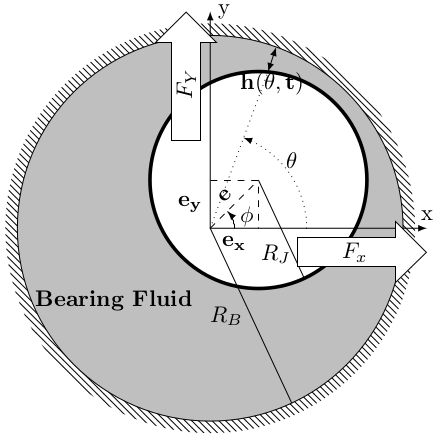
\includegraphics[width=\linewidth]{Figs/JB}
      \end{figure}
    \end{column}
    \begin{column}{0.5\textwidth}
      Required,
      \begin{eqnarray*}
        \begin{Bmatrix}F_X\\F_Y\end{Bmatrix}
      \end{eqnarray*}
      and derivatives $\pdderiv{e_x}$, $\pdderiv{e_y}$,
      $\pdderiv{\dot{e_x}}$, and $\pdderiv{\dot{e_y}}$
    \end{column}
  \end{columns}

  \begin{equation*}
    \begin{split}
      F_r &= -\mu RL{\left(\frac{L}{c}\right)}^2 \left[
        (\omega-2\dot{\phi}) \frac{\epsilon^2}{{(1-\epsilon^2)}^2} +
        \frac{\pi}{2}\frac{(1+2\epsilon^2)\dot{\epsilon}}{{(1-\epsilon^2)}^{5/2}}
      \right]\\
      F_t &= \mu RL{\left(\frac{L}{c}\right)}^2 \left[ (\omega-2\dot{\phi})
        \frac{\pi}{4}\frac{\epsilon}{{(1-\epsilon^2)}^{3/2}} +
        \frac{2\epsilon\dot{\epsilon}}{{(1-\epsilon^2)}^2} \right]
    \end{split}
  \end{equation*}
  \vspace{-0.5cm}
\begin{lstlisting}[basicstyle=\small]
depends([e],t)$
ex:0.3*50.8e-6*cos(%pi/4)$
ey:0.3*50.8e-6*cos(%pi/4)$
exd:0.1*ex*omega$
eyd:0.1*ey*omega$
epsilon:sqrt(e[x]**2+e[y]**2)/c$
phi:atan2(e[x],e[y])$

Fr:-mu*R*L*(L/c)**2*((omega-2*diff(phi,t))*
epsilon**2/(1-epsilon**2)**2 + %pi*(1+2*epsilon**2)*
diff(epsilon,t)/(2*(1-epsilon**2)**(5/2)))$

Ft:mu*R*L*(L/c)**2*((omega-2*diff(phi,t))*
% pi*epsilon/(4*(1-epsilon**2)**(3/2)) +
2*epsilon*diff(epsilon,t)/(1-epsilon**2)**2)$ 

Fx:radcan(Fr*cos(phi)-Ft*sin(phi))$
Fy:radcan(Fr*sin(phi)+Ft*cos(phi))$

FxFy:transpose(matrix([Fx,Fy]))$
\end{lstlisting}
\begin{lstlisting}[basicstyle=\small]
vals:[mu=0.00689,c=50.8e-6,L=12.7e-3,R=25.4e-3,
diff(e[x],t)=exd,diff(e[y],t)=eyd,e[x]=ex,e[y]=ey,
omega=10000*2*%pi/60]$

float(subst(vals,FxFy));
float(subst(vals,diff(FxFy,e[x])));
float(subst(vals,diff(FxFy,e[y])));
float(subst(vals,diff(FxFy,diff(e[x],t))));
float(subst(vals,diff(FxFy,diff(e[y],t))));

\end{lstlisting}
\end{frame}

\begin{frame}[fragile,allowframebreaks]
  \frametitle{Setting up imaxima on emacs}
  \begin{footnotesize}
\begin{verbatim}
(add-to-list 'load-path "/usr/share/maxima/5.37.2/emacs")
(autoload 'maxima-mode "maxima" "Maxima mode" t)
(autoload 'imaxima "imaxima" 
        "Frontend for maxima with Image support" t)
(autoload 'maxima "maxima" "Maxima interaction" t)
(autoload 'imath-mode "imath" 
        "Imath mode for math formula input" t)
(setq imaxima-use-maxima-mode-flag t)
(add-to-list 'auto-mode-alist '("\\.ma[cx]" . maxima-mode))
(setq imaxima-fnt-size "Large")

(autoload 'emaxima-mode "emaxima" "Emaxima" t)
(add-hook 'emaxima-mode-hook 'emaxima-mark-file-as-emaxima)
(setq emaxima-abbreviations-allowed t)
\end{verbatim}
  \end{footnotesize}

  \begin{figure}
    \centering
    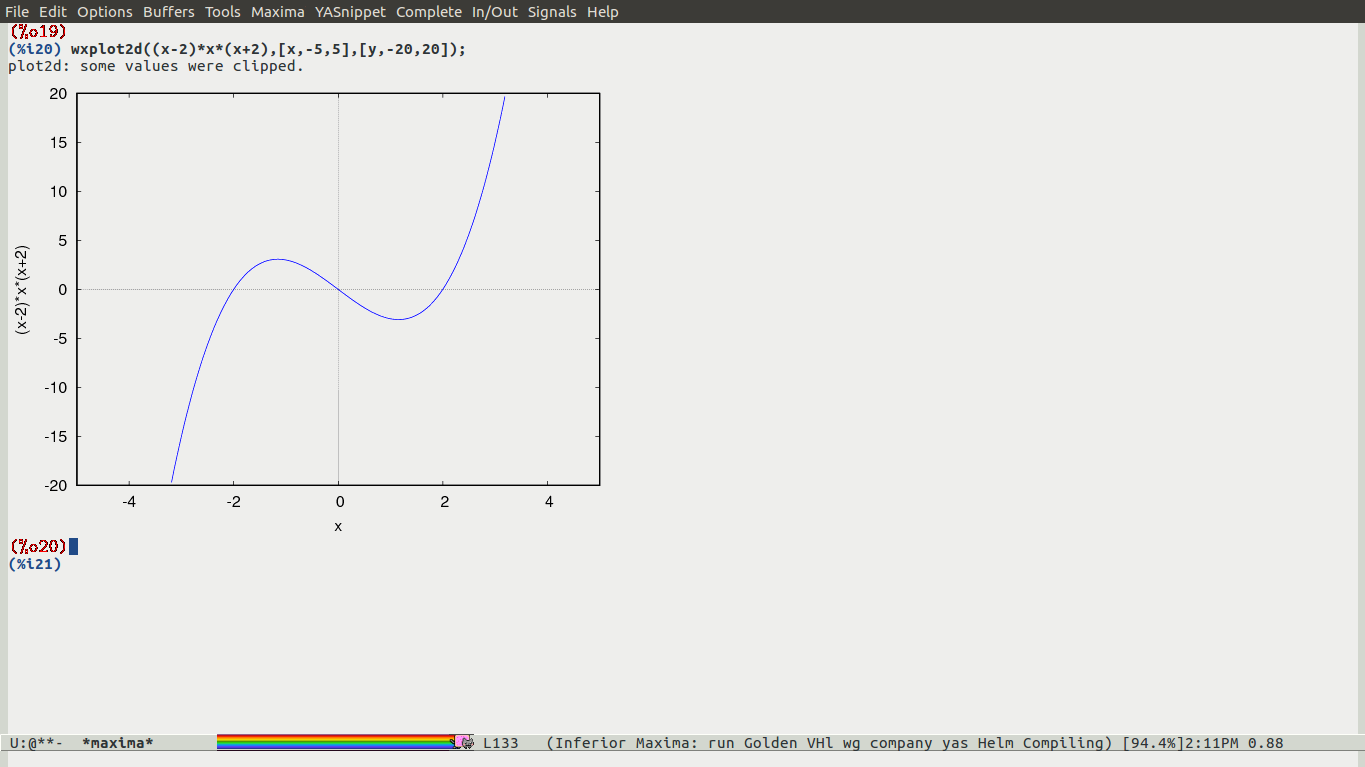
\includegraphics[width=\linewidth]{Figs/imaxima_demo}
  \end{figure}
\end{frame}

\begin{frame}[fragile]
  \frametitle{Useful Links}
  \begin{enumerate}
  \item \url{http://maxima.sourceforge.net/}
  \item \url{https://sourceforge.net/projects/wxmaxima/} (recommended
    front end)
  \item \url{http://web.csulb.edu/~woollett/} (great resources)
  \end{enumerate}
\end{frame}

\begin{frame}
  \frametitle{Thank You!}
  \begin{center}
    \begin{block}{Nidish Narayanaa B}
      Semester VIII,\\
      B.Tech. Aerospace Engineering, IIST\\
      +91-9496882251\\
      nidbid@gmail.com
    \end{block}
  \end{center}
\end{frame}

\end{document}

%%% Local Variables:
%%% mode: latex
%%% TeX-master: t
%%% End:
